\begin{comment}
The fact that a large number of high-performance
applications are written in C/C++ indicates the attraction and
potential of translating programs in these languages to dataflow
designs to improve performance and energy efficiency. Once the
dataflow design for a particular application has been generated, it is
optimised for the target architecture to maximise performance subject
to constraints such as latency, power consumption or cost.  Even when
performed manually, this approach can result in significant
performance improvements. Therefore, enhancing productivity of
developers using this approach would have a significant impact and is
exactly what this project would address.

\subsection{Motivation}


The translation and optimisation process is laborious and involves
many manual, slow and error-prone steps, that can include even a
complete redesigning of the original algorithm. Additionally,
high-performance applications rely heavily on complex architecture
specific optimisations. Transformations that enable hardware/software
partitioning \cite{Lam:Coutinho:Luk:2008}, low level optimisations
(e.g. operator bit width \cite{Cardoso:Diniz:Weinhardt:2010}) or high
level optimisations (such as loop unrolling \cite{aho1977principles},
blocking and tilling \cite{wolfe1995high}) obscure the application's
original purpose, reducing maintainability. Furthermore, since some
optimisations depend on platform specific properties (e.g. bit width
of Digital Signal Processors), mixing them with the application code
affects portability, complicating the process of targeting different
platforms without repeating the optimisation process. Finally, due to
the large number of design choices, an incomplete manual exploration
can lead to sub-optimal results. Considering these issues in the
context of cloud computing solutions that are expected to provide
heterogeneous acceleration for a plethora of customer applications,
the need for fully automated and portable code generation for
high-performance designs becomes apparent. In addition, the ability to
automatically explore various trade-offs between price, performance
and energy efficiency would provide cloud owners with flexibility in
implementing their business offering.

Hence it is important to decouple these transformations from the
application logic, allowing them to be reused on multiple platforms
and facilitating design space exploration. Using Aspect Oriented
Programming \cite{Kiczales:Lamping:Mendhekar:Maeda:Lopes:1997}, this
can be achieved by separating cross-cutting concerns, such as
optimisations and structural transformations, from the main algorithm
and encapsulating them in separate aspect descriptions.  Additionally,
aspect descriptions can be used to capture non-functional requirements
which may include constraints on power consumption, data rate,
latency, execution time etc. For example in a cloud computing
environment which manages many applications simultaneously, automated
optimisation techniques based on aspect descriptions can be used to
adapt implementations to fit long or short term power and performance
goals. These strategies could exploit the run-time reconfiguration
potential of FPGA chips to vary between existing implementations based
on input characteristics, or map the applications to different
accelerators.

Hence, the importance of the project lies in the potential to:
\begin{enumerate}
\item \textbf{improve performance of existing imperative applications
  by orders of magnitude}, by automating the translation to FPGA
  dataflow designs and providing an automated aspect-driven framework
  for exploring the design space of optimisation techniques applicable
  to fully customisable acceleration devices;

\item \textbf{address portability issues of massively parallel
  applications}, by using a novel aspect-driven synthesis flow which
  allows specification of platform independent optimisation
  strategies, possibly addressing global challenges in Exascale
  computing by allowing a portable expression of parallelism and data
  locality \cite[pp. 46 -- 50]{amarasinghe2009exascale};

\item \textbf{greatly increase developer productivity}, by automating
  the translation and optimisation process thus removing the potential
  for human error and facilitating the reuse of portable designs and
  optimisation strategies which could significantly reduce development
  time, given the lengthy compilation process on high-end FPGA devices
  \cite[pp. 23 -- 28]{Chen:Cong:Pan}.
\end{enumerate}

Consequently, the project could significantly improve performance of
state of the art dataflow designs and simplify the development and
maintenance of applications in key areas where high-performance
dataflow computing is used such as finance \cite{6339256,
  Weston:Martin:Spooner:Pell:Mencer:2010}, geoscience \cite{6226384},
weather forecasting \cite{Oriato:Tilbury:Marrocu:Pusceddu:2012} and
cloud computing \cite{710029}.

\section{Challenges}

\label{sec:intro-challenges}

Combining the dataflow paradigm with an aspect driven synthesis
flow could be expected to result in improved performance, portability
and developer productivity.  We believe that the following challenges
need to be addressed to facilitate the adoption of dataflow designs:

\begin{enumerate}

\item \textbf{Specifying dataflow designs}, in an intuitive, well
  understood language that is concise, facilitates the translation of
  existing designs, and is sufficiently expressive to support the
  requirements of modern high-performance applications. Compared to
  the solution used in
  \cite{Cardoso:Teixeira:Alves:Nobre:Diniz:Cutinho:Luk:2012}, this
  requires significant structural transformations to be captured and
  applied via aspect descriptions to transform the original imperative
  source into a dataflow implementation. However, results show that
  significant speedups can be achieved by targeting streaming
  architectures \cite{Pell:Mencer:2011}.

\item \textbf{Specifying optimisation strategies}, decoupled from the
  application code in a manner that makes the specification easy to
  reuse and to customise, and is comprehensive enough to allow
  capturing of optimisations at various levels: \emph{algorithmic
    transformations} of the original application that expose
  parallelism or improve communication between CPU and accelerator,
  \emph{design-level transformations} that enable exploration of
  platform specific optimisations and \emph{productivity related
    transformations} that improve developer productivity. Existing
  implementations for streaming architectures often require intricate
  specialisation steps to adapt and optimise the original
  application. These can be encapsulated in aspect descriptions and
  reused for multiple applications, simplifying the design process.
  For example, \cite{Xinyu:Qiwei:Luk:Qiang:Pell:2012} shows that using
  run-time reconfiguration to swap an application's idle sections with
  useful functions at run-time can lead to a 45\% performance
  improvement. Aspect-driven synthesis could be used to automate this
  optimisation, enabling its application for a broader class of
  programs.

\item \textbf{Systematic design space exploration} of dataflow designs driven
  by these parameterizable optimisation strategies, that increase
  developer productivity and allow exploration of design level
  trade-offs.

\item Applying these design techniques to \textbf{create and optimise
  high-performance applications}.

\end{enumerate}

In this project we investigate how these challenges can be addressed
by using an aspect-driven synthesis and optimisation process to
improve both design performance and designer productivity. This is
achieved by allowing the specification of reusable optimisation
strategies, and decoupling them and platform specific transformations
from the original application making it easier to maintain and more
portable. We study how techniques of Aspect Oriented Programming can
be applied to the compilation and optimisation of designs targeting
streaming Data Flow Engines (special computing devices built around
Field Programmable Gate Array chips that implement the dataflow
paradigm of computation). This includes identifying efficient compiled
patterns for streaming DFEs and how such patterns can be obtained from
high level descriptions using AOP design techniques.

We identify the following objectives:

\begin{enumerate}
\item \emph{Introduce a design flow that can be applied to integrate
    dataflow tools for FPGAs with flexible aspect weaving and design
    space exploration tools}
\item \emph{Identify novel aspect descriptions that enable design
  space exploration of dataflow designs from high level
  descriptions}.

\item \emph{Capture dataflow and platform specific optimisations
  using aspect descriptions and apply them to the generated
  designs}.

\item \emph{Evaluate the approach by implementing advanced
  high-performance applications}.
\end{enumerate}

In the next section we identify how these objectives can be met.

\section{Contributions}

We propose a methodology for addressing the challenges and meeting our
objectives based on the following contributions:

\begin{enumerate}

\item We propose a novel, automated method for design space
  exploration of dataflow designs, driven by optimisation and
  transformation strategies captured with aspect descriptions. This
  design flow is introduced in \cref{sec:design-flow}.

\item We introduce \FAST{}, a novel dataflow language based on C99
  syntax that can be used to create high-performance designs. The
  language is used as part of the proposed design flow to implement
  dataflow kernels. \Cref{sec:fast} provides an overview of the
  \FAST{} language.

\item We present novel aspects for specifying optimisation strategies
  at the system level, the implementation level, the exploration level
  and development level. We implement these aspects using
  LARA, an
  aspect oriented language for embedded reconfigurable systems. We present
  the aspect descriptions in \cref{sec:aspects}.

\item We implement a compiler that translates designs in \FAST{} to
  MaxCompiler designs which are then compiled and
  executed on a Maxeler MaxWorkstation containing a MAX3 DFE with a
  Virtex 6 FPGA chip and 24GB of DRAM.. We present an overview
  of our implementation in Chapter \ref{sec:implementation}.

\item We evaluate our approach by implementing a high-performance
  design for an application based on the Reverse Time Migration
  technique for seismic imaging
  \cite{Xinyu:Qiwei:Luk:Qiang:Pell:2012}. We discuss the results in
  Chapter \ref{sec:evaluation}.
\end{enumerate}

\begin{comment}
\section{Published Work}

As part of the project a full paper has been accepted for publication
at the 24th IEEE International Conference on Application-specific
Systems, Architectures and Processors, ASAP
2013\footnote{\url{http://asap-conference.org/}}.  The paper ``Aspect
Driven Compilation for Dataflow Designs'' \cite{pgrig} is based on
material from Chapters \ref{sec:design-flow}, \ref{sec:fast} and
\ref{sec:aspects} of this report and introduces the proposed design
flow, the FAST language and a number of aspect descriptions for
improving productivity and analysing resource trade-offs.

A second full paper is being drafted for submission at the 2013
International Conference on Field-Programmable Technology, ICFPT
2013\footnote{\url{http://www.fpt2013.org/}}. This is based on material
from Chapter \ref{sec:aspects} and introduces aspect descriptions for
run-time reconfiguration.

Finally, the approach and software implementation described in this
report were included into the FP7\footnote{European Union Seventh
  Framework Programme} funded HARNESS Project.
HARNESS\footnote{\url{http://www.harness-project.eu/?page_id=21}} aims
to integrate heterogeneous computing resources into cloud platforms in
order to reduce energy consumption and increase performance and cost
effectiveness of key cloud application in areas such as finance and
geoscience. The \FAST{} language and \fastc{} compiler will be used in
the process of generating efficient dataflow implementations for key
algorithms based on cloud owner requirements.

In this chapter we introduce a novel design flow for creating
high-performance dataflow designs starting from C/C++ applications. We
explain the motivation and requirements for the proposed approach and
provide an overview of its three main components:
\begin{itemize}
\item the \emph{\FAST{} language}, used to express dataflow kernels
\item the \emph{aspect description repository} and \emph{weaver}, which group
  and apply the optimisation and transformation strategies encapsulate
  through aspects
\item the \emph{compilation backend}, used to generate FPGA bitstreams
  from dataflow designs and link the host code run-time
  application
\end{itemize}
We show how these three components can be integrated to produce an
automated design technique. We analyse the steps required to produce
an optimised design using the proposed approach and compare this with
alternative approaches using other start-of-the-art
technologies. Finally, we present an extension to our original
design-flow to support run-time reconfiguration.


\begin{comment}
\section{Overview}

Figure \ref{fig:design-flow-overview} provides a brief overview of the
proposed design flow. First a high level application is produced as
the input to our flow. This is then partitioned into a software part
and a hardware part to run on the dataflow accelerator. A dataflow
kernel is generated from the original description. Aspect descriptions
are used to control the optimisation process.

Thus the inputs to the design flow are:
\begin{itemize}
\item High-level source specification
\item Aspect descriptions for controlling the compilation process
\end{itemize}

\begin{figure}[!h]
  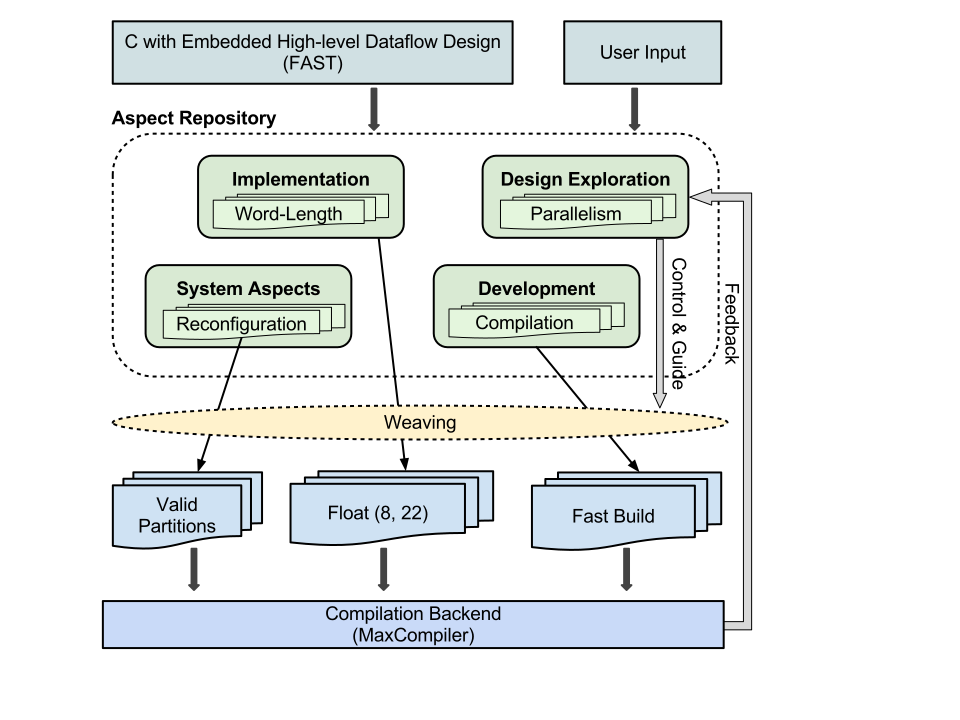
\includegraphics[scale=0.5, trim=60 50 0 0]{figs/asap13-design-flow.pdf_tex}
  \caption{Proposed approach for aspect-driven compilation of dataflow
    designs.}
  \label{fig:design-flow-overview}
\end{figure}
The design flow produces as its output a number of implementations based on
requirements specified through aspects.

The following algorithm describes the operation of the proposed design flow:

\begin{lstlisting}
  for (in as do als)
\end{lstlisting}

\end{comment}


\subsection{Performance and Energy Efficiency}
When targeting HPC applications it is crucial that our design flow
results in high-performance, highly efficient designs. By analysing
existing implementations for advanced high-performance applications
such as Reverse Time Migration (\Cref{app:rtm-kernel}), we identify key
requirements of these designs:

\begin{itemize}

\item \textbf{Computation is the most significant part} of
  high-performance applications. For stencil computations this is
  usually a fairly large stencil operation over a large number of
  adjacent data-points (multiple points in each dimension). For
  example, the RTM kernel uses two stencil operations of 31 floating
  point additions, 18 floating point multiplications and 1
  subtraction (\Cref{app:rtm-kernel}, Lines \ref{app:rtmk-op1} and
  \ref{app:rtmk-op2}).  Additionally, these are replicated
  \texttt{Par} times (with Par as large as 12) which leads to a total
  of $((31 + 18 + 1) * 2 * 12) = 1200 $ floating point operations to
  be executed on each kernel cycle (in reality floating point
  operations are pipelined across 13 kernel cycles, but this is,
  generally, transparent to the user). Hence, our approach must
  provide a clear and concise manner to express computation
  (preferably standard operators).

\item Another crucial aspect in achieving high-performance is
  \textbf{replicating the design} across the chip to maximise speedup
  subject to maximum available bandwidth. This makes use of FPGA cache
  (around 4MB of fast-local memory) to reuse data across time
  steps. This pipeline replication is achieved through design
  parametrisation and loops whose bounds are known at
  compile-time. The parameters that indicate the replication factor are
  shared across the compute and memory kernels but also across the CPU
  code.

\item High-performance designs \textbf{maximise usage of on-board
    DRAM}. Especially for stencil type computations where a number of
  time step iterations are performed over the original data, it is
  crucial to have the data available in the large, high bandwidth
  on-board DRAM rather than on the CPU side. Bandwidth of the on-board
  DRAM is 40GB/s compared to 2GB/s over PCI-Express to CPU. However,
  supporting DRAM introduces the additional complexity of managing
  multiple kernels (since memory read and write commands are,
  preferably, generated from kernels separated from the original
  dataflow kernel -- see \Cref{app:mem-read-kernel})
  and. Additionally, special API calls for generating the read/write
  commands have to be supported (\Cref{app:mem-read-kernel}, Line
  \ref{app:memrk-dram}).

\item \textbf{Expose optimisation opportunities for backend
  tools}. For example, our MaxCompiler backend supports some degree of
  trade-offs when mapping computation to DSPs. Additionally various
  trade-offs can be achieved by disabling pipeline depth etc.  These
  optimisations present interesting opportunities for trade-offs that
  enable developers to increase the number of parallel pipelines on
  the chip by balancing resource usage, or possibly reducing clock
  frequency.

\item Additionally, recent work shows the interesting possibility of
  improving design performance and energy efficiency for RTM by using
  run-time reconfiguration to remove idle functions has been recently
  showed that run-time reconfiguration can be used to improve the
  performance and energy-efficiency of FPGA designs. It is therefore
  important to facilitate the specification of strategies and designs
  that support run-time reconfiguration to maximise performance, both
  in the static flavour presented in
  \cite{Xinyu:Qiwei:Luk:Qiang:Pell:2012} where partitions are
  generated and scheduled optimally at compile-time but also in a
  dynamic, self-adaptive fashion \cite{6322875} in which the
  application can dynamically adapt itself by run-time reconfiguration
  based on input values.

\end{itemize}


\subsection{Productivity}

\subsubsection{Portability}

In the context of our design flow \emph{portability} refers to two
different aspects:
\begin{itemize}
\item \emph{portability of transformations and optimisations} -- it
  should be possible to reuse optimisation strategies in the context
  of different applications with as less user input as possible; in
  the context of RTM this is no longer possible: the transformation
  steps from the original naive implementation have been lost, and are
  now part of the existing code base. Of course these could be
  recovered, from version control for example, but a version control
  patch could obviously not be applied to other applications to
  generate highly pipelined designs. In other words if the developer
  was faced with the task of accelerating a similar computational
  kernel (which is likely since stencil computations follow a clear
  pattern) he would have to re-do all steps, resulting in a large
  decrease of productivity.

\item \emph{portability of designs over various FPGA devices} --
  generally resource available to FPGA chips vary greatly based on the
  chip manufacturer. Even in the simple case of chips produced by the
  same manufacturer, the reduction of a specific resource could
  prevent a design from working on a different FPGA chip. Hence
  designs cannot be considered portable, since a finely tuned design
  could not build on a different chip. By automating the design
  exploration process and identifying trade-offs automatically the
  optimisation process can be repeated for various devices without
  user input.
\end{itemize}

However, the issue of portability should not be restricted to the FPGA
design but also viewed in the context of the entire system
architecture. For example, as explained in
\Cref{sec:run-time-reconfiguration}, performance of run-time
reconfiguration designs also depends on characteristics such as data
transfer time and latency or whether partial reconfiguration is
possible.


%\XXX{Formulae for cost of automatic optimisation including design
%  space exploration and compute cost vs cost of manual developer
%  intervention}

\subsubsection{Integration}

It is important to facilitate the integration of application code
resulting from our approach with existing application code. For this
it should be possible to switch seamlessly between existing software
only code and dataflow based solutions. This can be achieved for
example by using pragmas or providing compiler extensions that when
enabled, indicate that a solution should be mapped to a dataflow
accelerator and indicate how to link hardware and software.

Integration is also required between the dataflow design running on
the accelerator and run-time API running on the host system. For
example, in the case of parallel replication of dataflow kernels, the
number of parallel processing pipelines needs to be known by both
components. This concern applies to other design parameters such as
word length, or run-time inputs. This suggests that there is a need to
synchronise these parameters to ensure correct operation. For example
the \texttt{Par} variable in the RTM kernel (\Cref{app:rtm-kernel},
Line \ref{app:rtmk-par}) contains the number of parallel pipelines
that are to be implemented in the design. Increasing the parallelism
reduces the number of cycles for which the kernel needs to executed.
Parameters sharing can be implemented via parameter files, but is
simplest when both components are written in the same language.

For example using C99 syntax, FAST would be able to share configuration
parameters with the CPU code (e.g. via constants or macro
definitions), simplifying management and integration of the CPU and
dataflow kernel.

\subsubsection{Automation}

Automating the design space exploration process results in
productivity improvements. However we provide input points in our
design flow which can be used gradually to tweak and guide the
compilation process.


On top of MaxCompiler, Maxeler offers a domain-specific compiler for
finite difference applications, MaxGenFD\cite{MaxelerFD}. This
simplifies the creation of finite difference kernels (such as those
required for the stencil applications described in
\Cref{sec:stencil-comp}). Although this abstracts effectively the
creation and optimisation of stencils, the process is not transparent
to the users and cannot be exposed to external design space
exploration tools. Like MaxCompiler, MaxGenFD provides no specific
support for designs with run-time reconfiguration.

\section{Extensions}

To support run-time reconfiguration effectively, the design flow of
\Cref{fig:design-flow} should be extended to support modelling and
recording of design resource usage, execution time, latency and power
metrics. These data are required when writing strategies for run-time
reconfiguration.

\subsection{Design Modelling}

A design model for resource usage, pipeline depth and timing
information can be created using limited user input. This is to be
used in the run-time reconfiguration to determine optimal partition
scheduling. Alternatively this information can be extracted from
portable platform description files such as those used in HARNESS
which contain a detailed specification of platform characteristics.

\begin{figure}[!ht]
  \centering
  \def\svgwidth{45em}
  \input{figs/rep-modelling.pdf_tex}
  \caption{High-level aspects controlling generation of design
    resource, performance and timing modelling.}
  \label{fig:reconfig-design-flow}
\end{figure}

Based on this model we can estimate design performance, latency,
energy efficiency and compilation time, and provide useful feedback
earlier in the development process than is possible with existing
tools.

Of course our model relies on user inputs for resource usage map
relies on estimates for resource usage and will not be expected to
provide very accurate results, especially in the presence of
optimisation of backend tools and various trade-offs that can be made
when mapping arithmetic to FF/LUT pairs vs DSPs.

\subsection{Run-time Reconfiguration Support}

In the proposed design flow we distinguish between:
\begin{itemize}
\item \textbf{static run-time reconfiguration} -- where partitions can
  be statically scheduled at compilation time after the design space
  exploration process has completed
\item \textbf{adaptive run-time reconfiguration} -- where partitioning
  depends on user input and an optimal schedule cannot be generated at
  compile time
\end{itemize}

Supporting both types of reconfiguration requires the introduction of
an additional modelling step which is performed prior to the
application of transformations for run-time
reconfiguration. Additionally a performance test suite is used to
measure and validate the results of partitioning.

Figure \ref{fig:reconfig-design-flow} presents an overview of the
revised design flow supporting run-time reconfiguration.

An additional requirement for adaptive run-time reconfiguration is a
configuration database where generated configurations and their
specification are stored for extraction, based on run-time
conditions.

\begin{figure}[!ht]
  \centering
  \def\svgwidth{\textwidth}
  \input{figs/fpt13-design-flow.pdf_tex}
  \caption{Revised design flow to support run-time reconfiguration}
  \label{fig:reconfig-design-flow}
\end{figure}

\begin{enumerate}
\item From an initial C + FAST design we create a number of
  configurations by applying implementation and system aspects as
  described in ASAP.
\item For each configuration we derive a model of the resource usage,
  performance and power usage using modelling aspects (described in
  section 3)
\item Based on predicted models (from step 2) and possibly on existing
  empirical information from the Design DB we partition the
  application and schedule the partitions to achieve user requirements
  and optimisation goals.
\item Finally a number of executables and designs are created,
  corresponding to the generated configurations from step 3. Based on
  compilation and execution (of automated performance tests) we refine
  our predictions for design resource usage, performance and power.
\end{enumerate}

Additionally the run-time environment has to be extended to support
this approach. An overview of the assumed runtime architecture for the
proposed approach is shown in Figure \ref{fig:reconfig-runtime}.

\begin{figure}[!ht]
  \centering
  \def\svgwidth{30em}
  \input{figs/fpt13-runtime.pdf_tex}
  \caption{Run-time architecture required to support run-time reconfiguration}
  \label{fig:reconfig-runtime}
\end{figure}

\begin{enumerate}
\item The CPU drives the FPGA. It initiates the computation and
  monitors the FPGA for factors such as temperature and power.
\item The CPU can request the FPGA to abort execution of the current
  design. Current results are saved (i.e. streamed back to CPU)
  before reconfiguration is triggered.
\item The CPU can select a new design to be uploaded
\item Empirical results are recorded in the Design Database, to
  improve future estimates of performance, power and thermal values.
\end{enumerate}

\section{Summary}

We have introduced the proposed Aspected-oriented design flow for
dataflow engines and introduced the components required to support
it. Optimisations are encapsulated in aspect descriptions, separated
from functional application code which leads to a more maintainable
and easier to understand programming model, with minimal impact on
performance. We show what extensions are required to the original
model in order to support the specification of strategies using
run-time reconfiguration to increase efficiency.

Compared to existing work described in
\cite{Cardoso:Teixeira:Alves:Nobre:Diniz:Cutinho:Luk:2012} and
\cite{cardoso2011new} our approach emphasises and provides more
freedom in the exploration of design level optimisation (such as word
length optimisations and mapping of arithmetic blocks to DSPs) by
using a combination of implementation aspects (shown in
\Cref{fig:design-flow}) and \FAST{} optimisation options.

\begin{comment}
Additionally, our approach targets a dataflow architecture as opposed
to the von Neumann architecture proposed in related work, which
typically includes a General-Purpose Processor (GPP) and a custom
accelerator. We consider additional optimisations to achieve
performance improvements as a result of a systematic design space
exploration process.

Compared to the MaxCompiler approach described in
\Cref{sec:back-maxcompiler}, the proposed design flow has a number of
benefits, the most exciting being the capability of capturing dataflow
designs using vanilla C and aspects. This is in direct contrast with
the meta-programming\cite{metaprogramming} approach used in
MaxCompiler which can be confusing to new users as suggested by many
queries on very basic matters from novice users on the Maxeler
Developer Forums\cite{mdx}. In addition, the MaxCompiler design
approach does not enable automating the design space exploration
process effectively. Because the dataflow design and run-time
component are written in different languages, integration with tools
for aspect weaving requires double the effort. The idea behind the
\FAST{} approach is to facilitate better integration with other tools
by providing a single language implementation. The reason behind using
meta-programming in MaxCompiler is to provide good support for design
parametrisation. In the \FAST{} approach this is achieved by
specifying optimisation strategies in the aspect descriptions,
simultaneously achieving the goals of decoupling optimisations form
application code and simplifying the programming model for dataflow
designs. This leads to improved productivity without affecting the
efficiency of the generated designs.
\end{comment}


The process of placing and routing a dataflow design can take anywhere
from 20 minutes to several days. Since this is a stochastic process,
usually mutliple builds are started in parallel and when one
terminates successfully the whole build process is stop and that
design is used. Hence the build process requires substantial amount of
DRAM and CPU cores, particulary during the design space exploration
step where multiple instances of the same design are compiled to
identify maximum performance configuration. Hence the builds were ran
on the Custom Computing cluster machines:

\begin{itemize}
\item \texttt{cccad3} -- 2 8 core, hyperthreaded (16 threads) Intel
  Xeon E5-2650 CPUs at 2.00GHz, 20MB cache, 189 GB DRAM
\item \texttt{cccad2} -- 2 6 core, hyperthreaded (12 threads) Intel
  Xeon X5650 CPUs at 2.67GHz, 12 MB cache, 94 GB DRAM
\item \texttt{cccad1} -- 2 6 core, hyperthreaded (12 threads) Intel Xeon
  X5650 CPUs at 2.67GHz, 12 MB cache, 118 GB DRAM
\end{itemize}

All CPU applications are compiled using GCC 4.4 with all optimisations
enabled (-O3 flag) and FPGA Designs are compiled with MaxCompiler
2012.1.


\begin{comment}
  In this section we outline the design goals of the
  language, introduce an early prototype and examine its advantages and
  limitations and propose an enhanced version. We highlight the main
  features of \FAST{} and explain how these translate to components of
  dataflow designs. We analyse the major challenges we met in creating
  the \FAST{} language and highlight the strategies we adopted for
  overcoming them.


  \section{Design Goals}


  \FAST{} is used to express the simplest form of a dataflow design
  while optimisations and other transformations are encapsulated in
  aspects which are developed separately and applied through aspect
  weaving. This results in a flexible approach for generating and
  exploring the space of efficient dataflow designs.

  Designs in \FAST{} are compiled to MaxCompiler designs composed of
  inter-connected functional kernels. Communication between kernels is
  asynchronous, so they can operate independently, and compute only when
  all active inputs have available data.

  \section{Features}

  We originally developed a simple prototype of the FAST language
  sufficient to support our application benchmark
  (\Cref{sec:benchmark}). We then extended this prototype with more
  advanced features (as described in \Cref{sec:fast-extensions}) which
  were required to meet our design goals.

  In this section we use a very simple implementation of a dataflow
  kernel which is part of our Black Scholes benchmark to highlight some
  of the main features of the \FAST{} language. This kernel simply
  computes the result of the finite difference approximation solution to
  the Black Scholes Equations, iterating both in space (the fast
  dimension -- stock prices) and in time (the slow dimension). In
  \Cref{sec:fast-ref} we analyse the same example in light of our
  extensions described in \Cref{sec:fast-extensions} and argue that
  these simplify the language.

  \lstset{style=MaxC}

  \begin{lstlisting}[
    label={lst:fast-bscholesp},
    caption={\FAST{} dataflow kernel for Black Scholes Options pricing}
    ]
    void Price_FPGA(s_float8_24 stockPrices,
    float8_24 c1, float8_24 c2, float8_24 c3,
    int32 nStocks, int32 stencilOrder, int timesteps)
    {
      // read input stream
      in(stockPrices);

      // counters for timestep and stockstep iteration
      int32 timestep  = count(timesteps, 1);
      int32 stockstep = countChain(nStocks, 1, i4);

      #pragma FAST DSPBalance:full
      s_float8_24 result =   stockPrices[ 0] * c1
      + stockPrices[ 1] * c2
      + stockPrices[-1] * c3;

      // boundary conditions for the stencil computation
      int32 up = (stockstep >= stencilOrder)
      && (stock < stockstep - stencilorder);

      // write output stream
      out(up ? result : stockPrices);
    }

    // Regular C style CPU implementation
    void Price_CPU(...) {...}

    int main() {
      #pragma FAST hw:Price_FPGA
      Price_CPU(...);
    }
  \end{lstlisting}

  Listing \ref{lst:fast-bscholesp} highlights some of the most important
  features of a \FAST{} dataflow kernel:
  \begin{itemize}
  \item dataflow kernels are declared as regular C functions with inputs
    defined as arguments in the function signature;
  \item streams are represented through \texttt{s\_<type>} types, which
    are type definitions for \texttt{<type *>}; these are interpreted
    as special types by the \fastc{} compiler;
  \item to provide easy access to previous, current and future stream
    values array notation is used with positive offsets accessing future
    values and negative offsets accessing previous stream values
  \item supported offset values are linear combinations of compile-time
    constants or variables (either loop induction variables,
    or normal variables but for which a compile time range of values is
    specified, as a requirement for generating efficient hardware)
  \item constructs such as loops are supported as long as their bounds
    are known at compilation time and are used to parametrise dataflow
    designs.
  \item C function calls are mapped to dataflow kernels via pragmas
    (Line 17) which provides the flexibility of selecting a particular
    dataflow configuration based on run-time conditions
  \end{itemize}


  Additionally and API is provided for higher-level constructs such as
  I/O functions (\texttt{in()}, \texttt{out()}), counters
  (Listing \ref{lst:fast-bscholesp}, Lines~4--5) and functions to multiplex
  streams (\texttt{mux()}).



  In the remainder of this section we provide an in-depth analysis of
  these features and design challenges associated with capturing them in
  a simple imperative language.

  \subsection{Kernels and Streams}

  \label{sec:kernels-streams}

  Kernels represent a unit of computation that is mapped to the FPGA.
  They are C functions that can be linked via pragmas placed before a
  corresponding CPU (non-accelerated) function call in the C
  application.  It is not convenient, or correct for that matter, to
  allow the direct calling of dataflow kernels. First of all, from the
  execution model point of view this would not make sense and would
  confuse the user since a ``call'' to the dataflow kernel more
  precisely maps to a sequence of calls where the data are streamed, one
  value per cycle, into the kernel and the stream counters are
  incremented at each kernel iteration (as shown in Algorithm
  \ref{alg:kernel-sim}).  Secondly, this can also lead to spurious
  warnings and even unexpected errors when compiling and running with a
  different compiler than \fastc{}.

  \begin{algorithm}
    \caption{Kernel Execution Loop}
    \label{alg:kernel-sim}
    \begin{algorithmic}
      \Function{RunKernel}{kernel, cyclesToRun}
      \State kInParams $\gets$ kernel.InputStreamPointers
      \State kOutParams $\gets$ kernel.OutputStreamPointers
      \State kConstantParams $\gets$ kernel.ConstantParams
      \State MAX\_CYCLE $\gets$ cyclesToRun
      \For{cycle $\in$ {1 ... cyclesToRun}}
      \State CURRENT\_CYCLE $\gets$ cycle
      \State call kernel(kInParams, kConstantParams)
      \For{streamPointer $\in$ kStreamParams}
      \State streamPointer $\gets$ streamPointer + 1
      \EndFor
      \EndFor
      \For{streamOutPointer $\in$ kOutParams }
      \State streamOutPointer $\gets$ streamOutPointer - cyclesToRun
      \EndFor
      \State \Return kOutParams
      \EndFunction
    \end{algorithmic}
  \end{algorithm}

  However, although disallowing direct calls to \FAST{} dataflow kernels
  enforces a more robust separation between the dataflow and CPU
  components, it introduces the complication of passing parameters to
  the kernel. We use the convention over configuration approach
  \cite{chen2006convention} to simplify parameter passing, assuming the
  following implicit mapping:
  \begin{enumerate}
  \item the first parameter of the CPU function call maps to the number
    of kernel cycles; this is mapped to a special variable named
    \texttt{MAX\_CYCLES} which is accessible within the dataflow kernel;
    it does not need to listed as a separate parameter in the kernel definition
  \item stream and constant parameters map to the identically named
    dataflow kernel parameters
  \item output streams are listed in identical order in the kernel
    function call as in the dataflow kernel design
  \item for situations where these conventions are not ideal, we provide
    the means of specifying parameter mappings using pragma parameters
    of the form \texttt{map:stream\_CPU, stream\_Kernel}.
  \item the special variable \texttt{CURRENT\_CYCLE} is updated with the
    current cycle count at each cycle as per Algorithm \ref{alg:kernel-sim}
  \end{enumerate}

  These conventions are illustrated in Listing \ref{lst:fast-kernel} and
  the resulting parameter mapping is explained in
  \Cref{table:fast-params}.

  \begin{table}[!ht]
    \begin{tabularx}{\textwidth}{X|X|c}
      \textbf{CPU Parameter} & \textbf{Dataflow Parameter} & \textbf{Explanation} \\
      \hline
      \hline
      n & MAX\_CYCLES & Rule 1 \\
      x &  a & Rule 4 \\
      y & y & Rule 2 \\
      y & s & Rule 2 \\
      prod & result1 & Rule 3 \\
      sum  & result2 & Rule 3 \\
      -- & CURRENT\_CYCLE & Rule 5
    \end{tabularx}
    \caption{Mapping of parameters from CPU function calls to \FAST{} dataflow kernel.}
    \label{table:fast-params}
  \end{table}

  Additionally we assume that all input and output streams and constant
  values are correctly allocated according to the C99 standard before
  the function call to the dataflow kernel is occurs.

  \begin{lstlisting}[caption={Simple \FAST{} dataflow kernel.}, label={lst:fast-kernel}]
    // standard C main function
    int main() {
      // allocate and pre-set x, y, prod and sum

      #pragma fast kernel:MovingAverage map:x, a
      MovingAverage(n, x, y, s, prod, sum);

      // do something useful with prod and sum
    }

    void MovingAverage(int32 *a, int32 *y, int32 s) {
      int32 result1 = a[0] * y[0] * CURRENT_CYCLE;
      int32 result2 = a[0] + y[0] + s;
      out(result1); out(result2);
    }
  \end{lstlisting}

  The kernel inputs can be streams or run-time constants. The kernel
  produces as output one or more streams of data. We distinguish between:

  \begin{itemize}
  \item \textbf{output/write stream}  -- allows access to previous and
    current values; write streams are created via calls to the
    \texttt{out} function as shown in Listing \ref{lst:fast-kernel};
  \item \textbf{input/read stream} -- allows access to previous, current
    and future values; these are the streams defined in kernel
    declaration (e.g. \texttt{a} and \texttt{y} in Listing
    \ref{lst:fast-kernel});
  \item \textbf{mixed output/input} streams -- allows access to
    previous, current and future values; mixed streams are streams that
    are defined within the kernel body.
  \end{itemize}

  \subsubsection{Stream Type}
  A key to obtaining high-performance FPGA designs is the use of custom
  data types, where the FPGA offers a higher degree of flexibility than
  the C implementation. We can for example create fixed point precision
  data types of arbitrary bit width for integer and fractional part or
  non-standard floating point formats. A key design space exploration
  step is that of identifying required data types based on application
  specific accuracy requirements. For example in the case of Reverse
  Time Migration decreasing operator width can result in dramatic
  improvements in performance (2 times faster) with unnoticeable effects
  on image quality \cite{hfu2010accelerate}.

  Hence, variable bit width integer, fixed and floating point data types
  should be supported. However, the C standard does not provide means to
  specify arbitrary width types \cite[pp. 33]{Cstandard}.  Although
  arbitrary bit width fields can be specified this can only be done
  inside \texttt{structs} and requires padding to a multiple of 8 bits,
  which severely limits and complicates the use of values defined in
  this manner.

  An alternative to the standard defined types is the introduction of
  custom type definitions. These can bear specific meaning to the
  \fastc{} compiler while remaining completely transparent to standard
  compilers such as GCC. This initial approach is illustrated in
  Listings \ref{lst:fast-kernel} and \ref{lst:fast-bscholesp}. A
  complete list of the type definitions and their corresponding C99 types
  is shown in \Cref{table:data-type}.

  \begin{table}[ht!]
    \begin{tabularx}{\textwidth}{c|c|c|X}
      \textbf{FAST Type}  & \textbf{C Type} & \textbf{Example} & \textbf{Explanation}                                                             \\
      \hline \hline
      float(exp)\_(mant)  & float           & float8\_22       & Single precision floating point value with 8 exponent bits and 22 mantissa bits  \\
      double(exp)\_(mant) & double          & double11\_50     & Double precision floating point value with 11 exponent bits and 50 mantissa bits \\
      fixed(exp)\_(mant)  & float           & fixed3\_12       & Fixed precision value with 3 integer bits and 12 fractional bits                 \\
      int(width)          & int             & int15            & Integer value with 15 bits                                                       \\
      uint(width)         & int             & uint15           & Unsigned integer value 15 bits                                                   \\
      s\_(type)           & type*           & s\_float8\_24    & Stream of single precision floating point values                                 \\
      s\_array\_(type)    & type**          & s\_array\_int32  & Stream array of integer values                                                   \\
    \end{tabularx}
    \caption{\FAST{} custom data type for variable bit width integer, fixed and floating-point values.}
    \label{table:data-type}
  \end{table}


  \subsubsection{Stream Offsets}

  Stream offset expressions are used to access previous or future stream
  values using the array index notation (as shown in Listing
  \ref{lst:fast-offsets}). These expressions should be linear
  combinations of compile time constants or constant inputs to the
  kernel. More efficient hardware can be constructed if bounds for the
  offset are specified. This can be done via the \texttt{pragma
    var:var\_name type:offset min:min\_value max:max\_value} shown on
  Line 1 of Listing \ref{lst:fast-offsets}.

  The array index notation offers a simple means of accessing stream
  values but introduces, for maintaining compatibility with the C
  standard to annotate all stream variables. For example this leads to
  the superfluous \texttt{x[0]} on Line 3 of Listing
  \ref{lst:fast-offsets}. In the context of large dataflow kernels it
  can be tedious and error-prone to annotate stream values so we
  introduce the possibility of declaring stream values as regular scalar
  (non-pointer/array) types. For example, on line 4 of Listing
  \ref{lst:fast-offsets}, the value of r can be used without need for
  annotation. This, however introduces the limitation that future or
  past values of the stream ``r'' cannot be accessed in the kernel
  anymore, as shown on Line 4.

  \begin{lstlisting}[caption={\FAST{} kernel using offsets.},label={lst:fast-offsets}]
    #pragma fast var:off type:offset min:-128 max:128
    void (int32 *x, int32 off) {
      int32 r = x[-off] + x[off] + x[1] + x[-1] + x[0];
      int32 o = 2 * r + 5;
      // int32 o = 2 * r[-1] + 5;  -- Illegal!
      out(o);
    }
  \end{lstlisting}


  \subsection{Control and Computation}

  Regular control statements can be used. When conditionals are based on
  stream values, the control statements are mapped by \fastc{} to
  hardware multiplexers.

  It is only possible to use loops statements (while, for) if their
  bounds and induction variables are known at compile time. In Listing
  \ref{lst:fast-compute-control} the loop is used to generate parallel
  arithmetic pipelines for every pair of inputs followed by an adder
  tree that reduces the result.

  Computation is captured using a mix of C operators and standard
  functions:
  \begin{itemize}
  \item C arithmetic operators can be used as usual on stream values (not streams themselves);
  \item C math.h function calls are automatically mapped to efficient hardware blocks;
  \item Arithmetic on streams (equivalent of pointer arithmetic) is
    illegal. Instead stream values must be extract by use of the current
    values operators (* or [0]).
  \end{itemize}

  \begin{lstlisting}[caption={Compute and control example in \FAST{}}, label={lst:fast-compute-control}]
    // constants can be used for design parametrisation
    const int nPairs = 2;

    void PairwiseSquareRootSum(s_array_float8_24 x) {
      float8_24 prod, sum;

      // loop is used for design parametrisation
      for (int i = 0; i < nPairs; i++) {
        prod = x[2 * i][0] + x[2 * i + 1][0];

        // C99  arithmetic functions can be mapped to hardware blocks
        sum = sum + sqrt(abs(prod));
      }
      out(sum);
    }
  \end{lstlisting}

  \subsection{Pragmas}

  Pragmas are used to indicate information that pertains to the
  optimisation process rather than the functionality of an
  application. In particular they indicate:
  \begin{itemize}
  \item optimisation options exposed by the backend tools
  \item additional type information required to generate variable width
    representations of operands
  \end{itemize}

  One exception is the hardware software linkage pragma which maps a
  software call to its corresponding dataflow engine version.

  The use of pragmas enables users to switch seamlessly between
  compilers and, eventually backend compilers, contributing towards the
  Integration requirement of our design flow.

  However, unlike in other approaches pragmas are not
  meant to be inserted manually -- although this is possible -- but
  rather they are to be controlled by the corresponding aspect
  descriptions (for hardware / software partitioning, optimisation
  etc.). The use of pragmas enables aspect descriptions to operate
  correctly (or rather to not operate incorrectly) accross various
  platforms (since, by definition, compiler directives are simply
  ignored if they are not understood by the compiler) and contributes
  towards our Portability requirement.

  Pragams in \FAST{} follow the syntax:

  \texttt{\#pragma fast (param\_name:param\_value)* (func:func\_name)?}

  The function name parameter simplifies loading of pragma information
  into a global data structure.

  \section{Extensions}

  \label{sec:fast-extensions}

  In this section we present the extensions we implemented on top of our
  \FAST{} and \fastc{} prototype in order to improve ease of use and
  simplify the language as much as possible. This simplifies adoption by
  users and also integration with the Harmonic Aspect weaver.

  \subsection{Inferring Stream Type}
  \label{sec:inf-stream-type}

  Our original approach to specifying variable stream types is
  problematic since it fails to decouple effectively the variable bit
  width optimisation from the application code. This in turn can lead to
  complications when writing aspect descriptions for exploring the
  design space of bit width optimisations since a more intensive
  analysis of the entire application is required in order to recognise
  optimisation pointcuts and generate correct designs when attempting to
  vary the representation of certain operands.

  To handle this situation we observe that, in general to classes of
  types are interesting to vary:
  \begin{itemize}
  \item I/O type -- this is the representation of a stream that when
    interfacing with the CPU; this has to be a standard C type to avoid
    data corruption
  \item kernel/compute type -- this the representation of a stream used
    inside the dataflow kernel, and hence, on the FPGA dataflow
    engine. This can be varied freely to non-standard types subject to
    accuracy requirements
  \end{itemize}

  Hence we introduce the following pragma for IO \texttt{pragma fast
    var:stream\_name ioType:typeToUseForIOInterface
    computeType:typeToUseInsideKernel}. Such pragmas can be
  automatically inserted by the aspect weaver based on various
  optimisation strategies and can be easily compiled by \fastc{} into
  corresponding MaxCompiler designs.

  Additionally, the \fastc{} compiler can be extended to automatically
  infer input and output streams (without requiring superfluous calls to
  the \texttt{in()} and \texttt{out}) method calls based on the following rules:
  \begin{itemize}
  \item If a stream is assigned to at least once then it is a write stream
  \item If a stream is assigned to more than once, then this is an error
  \item If a stream is declared in the kernel header and not written
    to, then it is a read stream
  \item If a stream is declared within the body of the dataflow
    kernel, it is a read/write stream
  \end{itemize}

  \subsection{Multiple Kernel Support}

  Some designs may require more than one dataflow kernel. Indeed all the
  applications in our benchmark contain at least three kernels: one
  computational kernel, and two kernels for generating read and write
  commands for the on-board DRAM. This is a typical use case where one
  kernel is to perform operations asynchronously from the other: merging
  the command generator kernels with the computation kernel can lead to
  a congested design and very easily to a kernel freeze (the equivalent
  of a deadlock in software). Hence, a recurrent pattern is where a
  separate kernel is used to generate the memory command stream, which
  contains the addresses that are to be read from DRAM.

  To support this scenario, MaxCompiler uses the concept of a manager
  which specifies how kernels are instantiated and connected together to
  form a design (as described in \Cref{sec:back-maxcompiler}).

  To support this scenario in FAST we extend our original pragma
  notations to enable the specification of:
  \begin{itemize}
  \item correlation between input and output
  \item kernel instances
  \end{itemize}

  \subsection{Support Designs with DRAM}
  \label{sec:fast-dram}

  Designs described
  To support DRAM a dataflow design requires additional kernels that
  generate memory commands asynchronously from the computational kernel.


  \subsection{Run-time Reconfiguration Support}


  To support run-time reconfiguration \fastc{} must know that
  alternative partititions are to be generated for a function.
  Additionally, boilerplate code for trigerring the run-time
  reconfiguration needs to be added. This contains:
  \begin{itemize}
  \item code required to save current FPGA state -- this is required to
    prevent loss of data as a result of resetting the device as part of
    the run-time reconfiguration process
  \item code on the CPU side to upload the new configuration
  \item code on the CPU side to queue new input streams and start the
    computation
  \end{itemize}

  \section{Revised FAST Example}
  \label{sec:fast-ref}

  Listing \ref{lst:fast-bscholesr} shows the revised Black Scholes
  implementation with the revised FAST language. No API calls are
  required for the counters or state saving. Inputs and outputs are
  clearly declared in the kernel header and the compiler can
  automatically infer whether a parameter stream is input or output. The
  type width information is decoupled from the application code and can
  be added automatically via aspect generated pragma statements.

  Additionally, we can use FPGA DRAM (bandwidth of 40GB/s) as the source
  for data, not just PCI-Express (2GB/s) which is a major improvement in
  terms of I/O bandwidth. This is achieved through our DRAM extensions
  and the support for multiple kernel that allows us to fully specify a
  three kernel design that implements the required pricing computation.

  \lstset{style=MaxC}

  \begin{lstlisting}[
    label={lst:fast-bscholesr},
    caption={\FAST{} dataflow kernel for European Options pricing}
    ]
    // 1. both input and output streams are declared in kernel header
    // 2. no need for additional type definitions
    void Price_FPGA(float* stockPrices, float *r,
    ... /* same as before */)
    {

      // 3. CURRENT CYCLE value used instead of counter API
      int stockstep  = (CURRENT_CYCLE / n1) \% timesteps;

      #pragma fast DSPBalance:full
      int result = ....; /* same as before */;

      // 4. boolean types used for conditions
      bool up = ...; /* same as before */ );

      // 5. assigning to output stream automatically outputs value
      r[0] = up ? result : stockPrices;
    }

  \end{lstlisting}

\end{comment}

\end{comment}
